\section{tasks::sum\-Frames Class Reference}
\label{classtasks_1_1sumFrames}\index{tasks::sumFrames@{tasks::sumFrames}}
Inheritance diagram for tasks::sum\-Frames::\begin{figure}[H]
\begin{center}
\leavevmode
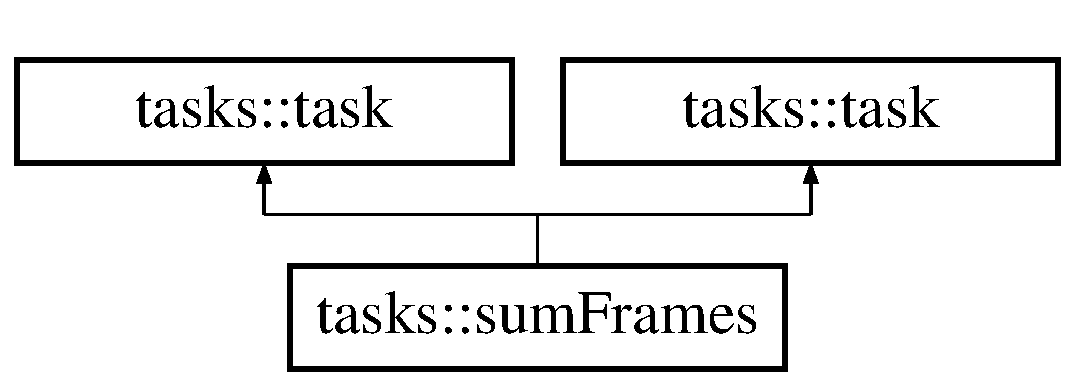
\includegraphics[height=2cm]{classtasks_1_1sumFrames}
\end{center}
\end{figure}
\subsection*{Public Member Functions}
\begin{CompactItemize}
\item 
def \textbf{run}\label{classtasks_1_1sumFrames_8505dc4d406e3855d5ea6f7ef62ea8f6}

\item 
def \textbf{run}\label{classtasks_1_1sumFrames_8505dc4d406e3855d5ea6f7ef62ea8f6}

\end{CompactItemize}
\subsection*{Static Public Attributes}
\begin{CompactItemize}
\item 
string \textbf{name} = '{\bfsum\-Frames}'\label{classtasks_1_1sumFrames_26a705fa0134ebed8b812a1869d5e29f}

\item 
string \textbf{button\-Text} = '{\bfsum\-Frames}'\label{classtasks_1_1sumFrames_6fe6d81705c571d117cbc4c0324b44bc}

\item 
int \textbf{inthread} = 0\label{classtasks_1_1sumFrames_75120b8d8397f28df2023c6736a2b734}

\end{CompactItemize}


\subsection{Detailed Description}


\footnotesize\begin{verbatim}A task for sum N frames
\end{verbatim}
\normalsize
 



The documentation for this class was generated from the following files:\begin{CompactItemize}
\item 
old/PANICtool-1.0/tasks.py\item 
old/tasks.py\end{CompactItemize}
